\newpage
\section{Ogólne określenie wymagań}

\begin{itemize}
	\item Aplikacja powinna korzystać z aktualnej lokalizacji użytkownika za pomocą GPS, aby wyświetlać najbliższe sklepy spożywcze żabka.
	\begin{figure}[!hbt]
		\begin{center}
			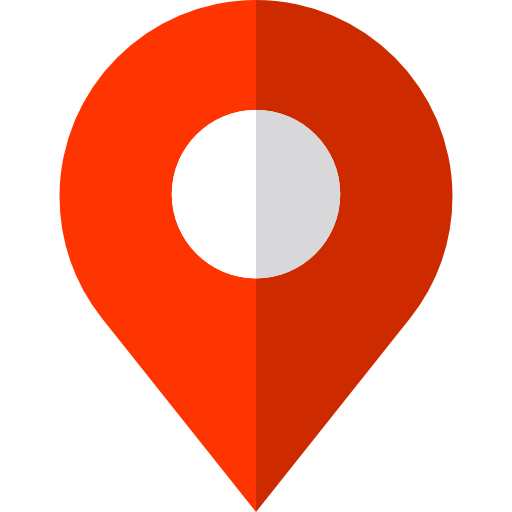
\includegraphics[width=4cm]{rys/gps-icon.png}
			\caption{Gps}
			\label{rys:ustawienia}
		\end{center}
	\end{figure}
	\item Użytkownik powinien mieć możliwość wyświetlania sklepów spożywczych na mapie wraz z ich odległością od aktualnej lokalizacji.
	\item Aplikacja powinna umożliwiać użytkownikom przeglądanie szczegółów sklepów, takich jak godziny otwarcia, dostępne produkty i oceny klientów.
	\item Klienci powinni mieć możliwość przesłania zdjęć produktów lub sklepu, co umożliwi innym użytkownikom ocenę sklepu spożywczego.
	\item Aplikacja powinna umożliwiać użytkownikom dodawanie recenzji i ocen sklepów spożywczych.
	\item Klienci powinni mieć możliwość zaplanowania trasy do wybranego sklepu spożywczego za pomocą nawigacji zintegrowanej z aplikacją.
	\item Aplikacja powinna wyświetlać informacje o dostępności produktów i cenach w poszczególnych sklepach spożywczych.
	\item Użytkownicy powinni mieć możliwość zapisywania ulubionych sklepów spożywczych i otrzymywania powiadomień o promocjach lub specjalnych ofertach.	
\end{itemize}

